% 1977 年甘肃卷第六题：圆台二视图（上：正视图等腰梯形，标 ∅20、∅60；
% 下：俯视图同心圆；竖直点划线为轴线，贯穿两视图，按源卷第 3 页布局）
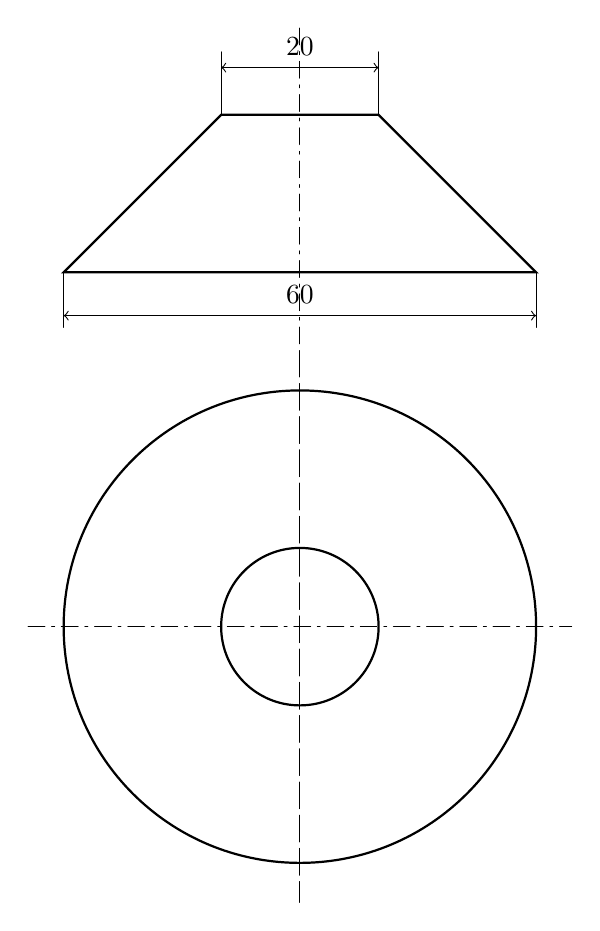
\begin{tikzpicture}[scale=0.5, line cap=round]
  % ---- 正视图：等腰梯形 ----
  \coordinate (TL) at (-2,13);
  \coordinate (TR) at (2,13);
  \coordinate (BR) at (6,9);
  \coordinate (BL) at (-6,9);
  \draw[thick] (TL)--(TR)--(BR)--(BL)--cycle;
  % 上口尺寸线 ∅20
  \draw[thin] (-2,13)--(-2,14.6);
  \draw[thin] (2,13)--(2,14.6);
  \draw[<->] (-2,14.2)--(2,14.2);
  \node[above] at (0,14.25) {$\varnothing 20$};
  % 下口尺寸线 ∅60
  \draw[thin] (-6,9)--(-6,7.6);
  \draw[thin] (6,9)--(6,7.6);
  \draw[<->] (-6,7.9)--(6,7.9);
  \node[above] at (0,7.95) {$\varnothing 60$};
  % ---- 竖直轴线（点划线，贯穿两视图）----
  \draw[dash pattern={on 6pt off 2.5pt on 1pt off 2.5pt}, thin]
        (0,15.2)--(0,-7);
  % ---- 俯视图：同心圆 ----
  \draw[thick] (0,0) circle (6);
  \draw[thick] (0,0) circle (2);
  \draw[dash pattern={on 6pt off 2.5pt on 1pt off 2.5pt}, thin]
        (-6.9,0)--(6.9,0);
  \draw[dash pattern={on 6pt off 2.5pt on 1pt off 2.5pt}, thin]
        (0,-6.9)--(0,7);
\end{tikzpicture}
